\documentclass{beamer}
\usepackage{amsmath}
\usepackage{graphicx}
\usepackage{url}
\usepackage{listings}
\usepackage{fancyvrb}
\usepackage[T1]{fontenc}
\usepackage{hyperref}
\usepackage{listings}
\mode<presentation>
%{ \usetheme{Warsaw} }
\title{ACA Summer School 2014\\ Advanced C\texttt{++}}

\setbeamercovered{transparent=5}

\author{Pankaj Prateek}
\institute{ACA, CSE, IIT Kanpur}
\date{\today}

\lstset{language=C++,
  basicstyle=\ttfamily,
  tabsize=3,
  keywordstyle=\color{blue}\ttfamily,
  stringstyle=\color{green}\ttfamily,
  commentstyle=\color{red}\ttfamily,
  morecomment=[l][\color{magenta}]{\#},
  backgroundcolor=\color{black!5},
  % basicstyle=\footnotesize,
}
 
\AtBeginSection[]  % "Beamer, do the following at the start of every section"
{
\begin{frame}<beamer> 
\frametitle{Outline} % make a frame titled "Outline"
\tableofcontents[currentsection]  % show TOC and highlight current section
\end{frame}
}

\begin{document}
%----------- titlepage ----------------------------------------------%
\begin{frame}
  \titlepage
\end{frame}

\begin{frame}[fragile]{Code Reusability}
  \begin{itemize}
  \item Nobody likes to write code for the same functionality again and again without any significant improvement\pause
  \item Using already written code is more reliable, saves time, money and frustration for the programmer while debugging\pause
  \item Example of reuse: for students and teachers, the properties of the class person are common, and hence should be implented only once\pause
  \item Reuse of class : Inheritance\pause
  \item Inheritance : Using old classes and their properties to make new classes\pause
  \item Old class : Base class\pause
  \item New class : Derived class\pause
  \item The derived class inherits, some or all, properties of the base class
  \end{itemize}
\end{frame}

\begin{frame}[fragile]{Inheritance}
  \begin{lstlisting}
class new_class : visibility_mode old_class {
  // Some stuff for new class
  // Nothing special
};
  \end{lstlisting}\pause
  \begin{itemize}
    \item Indicates that the new\_cass had been derived from the old\_class in the specified visibility mode.
  \end{itemize}
\end{frame}

\begin{frame}[fragile]{Inheritance}
  \item \alert{Only ``public'' members are inherited}. Private members of base class are never accessible to any derived class. They can be accessed indirectly using public members from the same base class.
\end{frame}

\begin{frame}[fragile]{Inheritance: Private}
  \begin{lstlisting}
class XYZ {
  // members of XYZ
}
class ABC : private XYZ {
  // members of ABC
}
  \end{lstlisting}\pause
  \begin{itemize}
    \item Privately inherited/derived: ``Public'' members of the base class become ``private'' members of the derived class\pause
    \item Thus the public members of XYZ inherited into ABC can only be accessed through public functions of ABC\pause
    \item As a result, the inherited members of the base class are not directly accessible to the objects of the derived class. Access is restricted to the public members only
  \end{itemize}
\end{frame}

\begin{frame}[fragile]{Inheritance: Private}
  \begin{lstlisting}
// Derived class in private Inheritance
// How it looks in concept
// NOT REAL!!!
class ABC: private XYZ {
private:
  ... private members of XYZ
  ... private members of ABC
public:
  ... public members of ABC
};
  \end{lstlisting}
\end{frame}

\begin{frame}[fragile]{Inheritance: Public}
  \begin{lstlisting}
class XYZ {
  // members of XYZ
}
class ABC : public XYZ {
  // members of ABC
}
  \end{lstlisting}\pause
  \begin{itemize}
    \item Publicaly inherited/derived: ``Public'' members of the base class become ``public'' members of the derived class\pause
    \item Thus the public members of XYZ inherited into ABC can be accessed directly by the objects of ABC
  \end{itemize}
\end{frame}

\begin{frame}[fragile]{Inheritance: Public}
  \begin{lstlisting}
// Derived class in private Inheritance
// How it looks in concept
// NOT REAL!!!
class ABC: private XYZ {
private:
  ... private members of ABC
public:
  ... public members of XYZ
  ... public members of ABC
};
  \end{lstlisting}
\end{frame}

\begin{frame}[fragile]{Inheritance: Protected}
  \begin{itemize}
    \item At times we may require that a private member be inherited by the derived class\pause
    \item An obvious way to achieve this is to make it public. But at the cost of losing the advantage of Data Hiding\pause
    \item Hence to facilitate this, C++ has a new keyword : protected\pause
    \item A ``protected'' member of a class, is accessible by the member functions within that class or any class ``immediately'' derived from it
  \end{itemize}
\end{frame}

\begin{frame}[fragile]{Inheritance: Protected}
  \begin{lstlisting}
class class_name {
private:
  // visible only to member functions 
  // of this class
protected:
  // visible only to member functions of 
  // this class and immediate derived class
public:
  // visible to all functions in the program
}
  \end{lstlisting}
\end{frame}

\begin{frame}[fragile]{Inheritance: Protected}
  \begin{itemize}
    \item The keyword protected is used in the same way public and private are used\pause
    \item With this, C++ also allows a protected mode of inheritance as well along with public and private\pause
    \item Private and protected members of a class can now be accessed by friend functions or member functions of a friend class
  \end{itemize}
\end{frame}

\begin{frame}[fragile]{Visibility of Inherited Members}
  \begin{table}
    \caption{Derived Class Members: Visibility}
    \begin{tabular}{|c|c|c|c|}\hline
      Declaration $\rightarrow$ & Private & Protected & Public\\\hline
      private & Not inherited & Not inherited & Not inherited\\\hline
      protected & Private & Protected & Protected\\\hline
      public & private & protected & public\\\hline
    \end{tabular}
  \end{table}
\end{frame}

\begin{frame}[fragile]{Multilevel Inheritance}
  \begin{itemize}
    \item It is when there is a series of inheritance from one class to its child class\pause
    \item The general rules of inheritance are followed as they are.\pause
      \begin{center}
        Class A\\ $\uparrow$\\ Class B\\ $\uparrow$\\ Class C
      \end{center}\pause
    \item Class B is also called intermediate base class of A\pause
    \item The chain A-B-C is called inheritance path
  \end{itemize}
\end{frame}

\begin{frame}[fragile]{Multiple Inheritance}
  \begin{itemize}
    \item A class can inherit from multiple classes. Hence called multiple inheritance\pause
    \item Allows the user to combine several features from different classes at the beginning of creating a new class\pause
      \begin{lstlisting}
class D: visibility B1, visibility B2 {
  // definition of D
};
      \end{lstlisting}\pause
    \item Visibility can be either public, private or protected.\pause
    \item This feature is quite unique to C\texttt{++}. Even JAVA doesn't support multiple inheritance.
  \end{itemize}
\end{frame}

\begin{frame}[fragile]{Multiple Inheritance}
  \begin{lstlisting}
class B1 {
public:
  int abc;
}
class B2 {
public:
  int abc;
}
class D: visibility B1, visibility B2 {
  // definition of D
};
  \end{lstlisting}\pause
  Class D will have two variables with the same name. Ambiguity!!!
\end{frame}

\begin{frame}[fragile]{Multiple Inheritance: Ambiguity Resolution}
  \begin{itemize}
    \item The ambiguity is only flagged as an error if you use the ambiguous member name.\pause
    \item You can resolve ambiguity by qualifying a member with its class name using the scope resolution (::) operator.
  \end{itemize}
\end{frame}

\begin{frame}[fragile]{Hierarchical Design}
  \begin{itemize}
    \item In the real world, the systems to be developed are far too complex in nature, and involve a lot of programming\pause
    \item Professional programming is done in stages\pause
    \item Beginning from the basic functionality, going up to the most advanced one\pause
    \item Code is written in the form of small modules\pause
    \item Sequences of inheritance starting from the most basic to the most advanced are slowly developed\pause
    \item Benefits : Modular design, ease of maintenance, clarity of thought, faster error localization
  \end{itemize}
\end{frame}

\begin{frame}[fragile]{Multipath Inheritance}
  \begin{center}
  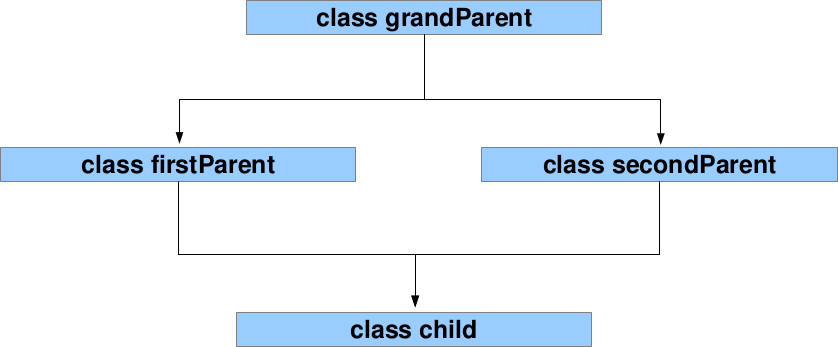
\includegraphics[scale=0.3]{lec.jpg}\pause
  \end{center}
  \begin{itemize}
  \item firstParent and secondParent, both inherit from grandParent\pause
  \item Child inherits from both the parents\pause
  \item Child now has two copies of every inherited member of grandParent
  \end{itemize}
\end{frame}

\begin{frame}[fragile]{A new keyword : ``virtual''}
  \begin{itemize}
  \item Problem: The child inherits the members of the grandparent twice\pause
  \item This problem can be solved by declaring the inheritance of common base class as virtual
  \end{itemize}
\end{frame}

\begin{frame}[fragile]{A new keyword : ``virtual''}
  \begin{itemize}
  \begin{lstlisting}
class grandParent {
  ...
};
class Parent1 : virtual public grandParent {
  ...
};
class Parent2 : virtual public grandParent {
  ...
};
class child : public Parent1, public Parent2 {
  ...
};
  \end{lstlisting}\pause
  \item C\texttt{++} checks that only one copy of the virtual base class is inherited.
  \end{itemize}
\end{frame}

\begin{frame}[fragile]{Abstract Class: Concept}
  \begin{itemize}
  \item Its a program design concept\pause
  \item A class which is designed to be specifically used as a base class\pause
  \item No concrete objects are created out of it.\pause
  \item It only represents the common basic properties of the derived classes\pause
  \item It has at least one pure virtual function. (explained later)\pause
  \item Any class derived from an abstract class will also be an abstract class if the virtual function is not defined.
  \end{itemize}
\end{frame}

\begin{frame}[fragile]{Constructors and Inheritance}
  \begin{itemize}
  \item Constructors : initialize new objects of a class\pause
  \item If there is no constructor in any base class, then derived class need not necessarily have a constructor of its own\pause
  \item However if any of the base classes has a constructor, then its mandatory for the derived class to have a constructor as well\pause
  \item Base class is a part of the derived class after inheritance.\pause
  \item Hence the derived class constructor should pass arguments to the base class constructor\pause
  \item Base class constructors executed first in order of appearance in the derived class defenition, followed by the derived class constructor
  \end{itemize}
\end{frame}

\begin{frame}[fragile]{Defining a constructor}
  \begin{itemize}
  \item Assume that the derived class is inherited from base classes 1 to N\pause
    \begin{lstlisting}
DerivedClass (List1, List2, ..., ListN, 
               ListDerived) :
BaseClass1(List1),

BaseClass2(List2),

BaseClass3(List3),

BaseClassN(ListN) {
  // body of constructor of the derived class
}
    \end{lstlisting}
  \end{itemize}
\end{frame}

\begin{frame}[fragile]{Defining a constructor}
  \begin{itemize}
  \item Constructors of the base classes are invoked in order of their appearance in the definition of the derived class
  \end{itemize}
\end{frame}

\begin{frame}[fragile]{Defining a constructor}
  \begin{lstlisting}
class A {
public:
  int temp1;
  A(int i);
};
class B {
public :
  float temp2;
  B(float j);
};
class C: public A, public B {
public:
  char temp3;
  C(int i, float j, char c): A(i), B(j) {
    temp3 = c;
  }
};
  \end{lstlisting}
\end{frame}

\begin{frame}[fragile]{Constructor: Initialization lists}
  \begin{itemize}
    \item C\texttt{++} provides an extra way to initialize a class via initialization list\pause
      \begin{lstlisting}
ConstructorName(Argument List) 
           : initialization section {
  // rest of the constructor definition
}
      \end{lstlisting}\pause
    \item The initialization occurs in the order of declaration, irrespective of the order in the list provided
  \end{itemize}
\end{frame}

\begin{frame}[fragile]{Constructor: Initialization lists}
  \begin{lstlisting}
class XYZ {
  int a, b, c;
public:
  XYZ(int i, int j, int k) 
           : a(i), b(i+j), c(i+j-k) {
    cout<<''constructor XYZ''<<endl;
  }
};
class ABC : public XYZ {
  int z;
public:
  ABC(int i, int j, int k, int l) 
           : XYZ(i,j,k), z(l) {
    cout<<''constructor ABC'';
  }
};
  \end{lstlisting}
\end{frame}

\begin{frame}[fragile]{Nesting of classes}
  \begin{itemize}
  \item Till now we saw that inheritance is a mechanism to extend the properties of one class to a new class\pause
  \item C++ provides a second mechanism for the same purpose, which is in some sense more intutive, but used less\pause
  \item This approach has the view that a new object can be formed by the collection of many other objects\pause
  \item For eg : A car is made up of an Engine, four wheels, Headlights etc\pause
  \item The objects of ``base class'' are directly used as ``members'' of the new class
  \end{itemize}
\end{frame}

\begin{frame}[fragile]{Nesting of classes}
  \begin{lstlisting}
class A {
  // definition of A
};
class B {
  // definition of B
};
class C {
  A objA;
  B objB;
  // definition of class C
}
  \end{lstlisting}\pause
  All objects of the class C will contain the objects of A and B
\end{frame}

\begin{frame}[fragile]{Nesting of classes}
  \begin{itemize}
  \item This sort of declaration or relationship between classes is called ``Nesting'' or ``Containership''\pause
  \item Such objects are created in 2 stages:\pause
    \begin{itemize}
    \item First the member objects are created using their own consrtuctors\pause
    \item Then rest of the ordinary members of the class are created
    \end{itemize}
  \end{itemize}
\end{frame}

\begin{frame}[fragile]{Nesting of classes: With Constructors}
  \begin{itemize}
  \item Since the member objects have to be created earlier, their constructors must be called earlier as well\pause
  \item This is accomplished by the initialization list method for constructors\pause
    \begin{lstlisting}
C(int x, float y, char z)
           : obj1(x), obj2(x,y,z) {
  // definition of the constructor
}
    \end{lstlisting}\pause
  \item The arguments in the initialization lists is for the member objects and not the respective classes\pause
  \item The arguments passed to the member objects may or may not be from the argument list input to the constructor\pause
\item The constructors of the member objects are called in the order of their declaration in the class definition and not as per the order in the list
  \end{itemize}
\end{frame}

%% \begin{frame}[fragile]{Pointer: Basics}
%%   \begin{itemize}
%%     \item Variable
%%       \begin{center}
%%         Name/Identifier $\leftrightarrow$ Contains a value $\leftrightarrow$ Memory address
%%       \end{center}\pause
%%     \item Memory cells are numbered in continuation, giving every cell a unique number, which is called its address\pause
%%     \item Pointer
%%       \begin{center}
%%         Name/Identifier $\leftrightarrow$ Contains memory address of another variable
%%       \end{center}\pause
%%     \item Pointers contain the address of some other variable. They are said to ``point to'' that variable
%%   \end{itemize}
%% \end{frame}

%% \begin{frame}[fragile]{Pointer: Basics}
%%   \begin{lstlisting}
%% int a;
%% int *ptr = &a; //Reference operator
%% a = 10;
%% *ptr = 12;   //Dereference operator
%%   \end{lstlisting}
%% \end{frame}

%% \begin{frame}[fragile]{Pointer: Basics}
%%   \begin{itemize}
%%     \item Pointers are type-specific (that is there is a different pointer for every different type of variable)\pause
%%     \item Pointer to a pointer is also possible (double reference)\pause
%%     \item Extremely useful in call by reference mechanism\pause
%%     \item Also useful in dynamic memory allocation\pause
%%     \item Void pointer : a type-less pointer, but cannot be dereferenced without explicit type cast\pause
%%     \item Null pointer : A pointer that points to nothing or 0. Cannot be derefrenced. Doing that raises a run-time error/segmentation fault\pause
%%     \item Equivalent array names
%%   \end{itemize}
%% \end{frame}

%% \begin{frame}[fragile]{Pointers to structures}
%%   \begin{lstlisting}
%% struct temp {
%%   int a; float b;
%% };
%% int main() {
%%   struct temp obj1;
%%   struct temp * ptr;
%%   obj1.a = 10;
%%   obj1.b = 3.14;
%%   ptr = &obj1;
%%   cout << ptr -> a << endl;
%%   cout << (*ptr).b << endl;
%% }
%%   \end{lstlisting}
%% \end{frame}

%% \begin{frame}[fragile]{Pointer Arithmetic}
%%   \begin{itemize}
%%     \item ++ and $--$ operators are alowed on pointers\pause
%%     \item They correspond to advancing and retreating the pointer by the size of one object in memory\pause
%%     \item + and - are also allowed on pointers, which advance or retreat them suitably\pause
%%     \item *(a + 10) is equivalent to a[10] while (a + 10) is equivalent to &a[10]\pause
%%     \item Should be used with caution. Can possibly be the result of array out of bounds errors, resulting in segmentation faults\pause
%%     \item Array names are treated as constant pointers. Operations like A = A+1 are invalid for them
%%   \end{itemize}
%% \end{frame}

%% \begin{frame}[fragile]{Pointer: Basics}
%%   \begin{itemize}
%%     \item References are alias (second name) to variables\pause
%%     \item They do not contain memory address like pointers do\pause
%%     \item Unlike pointers, once assigned, then cannot be changed later\pause
%%     \item There are no Null references. They have to be initialized when they are declared.\pause
%%     \item The actual pass by reference is implemented through them, passing pointers is still only pass by value
%%   \end{itemize}
%% \end{frame}

%% \begin{frame}[fragile]{Pointers to Objects}
%%   \begin{lstlisting}
%% class ABC {
%%   int var1;
%% public:
%%   setVar(int a);
%%   int getVar();
%% };
%% ABC obj1;
%% ABC* ptr1;
%% ptr1 = &obj1;
%% ptr1->setVar(20);
%% cout<<ptr1->getVar();
%%   \end{lstlisting}
%% \end{frame}

%% \begin{frame}[fragile]{Pointers to Objects}
%%   \begin{itemize}
%%     \item Obviously, private data members cannot be accessed through pointers.\pause
%%     \item Way to access the public members is exactly like that in structures\pause
%%     \item The type checking of pointers is slightly loose in some sense when it comes to classes
%%   \end{itemize}
%% \end{frame}

%% \begin{frame}[fragile]{Pointers to Objects of derived class}
%%   \begin{lstlisting}
%% class ABC {
%%   int var1;
%% public:
%%   setVar(int a);
%%   int getVar();
%% };
%% class XYZ: public ABC {
%% int var2;
%% public:
%%   void setVar2(int b);
%%   int getVar2();
%% };
%% ABC obj1;
%% ABC* baseptr;
%% XYZ obj2;
%% baseptr = &obj1;
%% baseptr = &obj2;
%%   \end{lstlisting}
%% \end{frame}

%% \begin{frame}[fragile]{Pointers to Objects of derived class}
%%   \begin{itemize}
%%     \item Derived class object also contains a part of itself as the Base class\pause
%%     \item Hence, a pointer to base class can also point to an object of the derived class\pause
%%     \item But such a pointer can point only to the part of the derived class which houses the base class\pause
%%     \item To access member of the derived class, we need an explicit pointer to the derived class\pause
%%     \item Even when using a base class pointer for a derived class object, only the inherited members are accessible and not the whole class
%%   \end{itemize}
%% \end{frame}

%% \begin{frame}[fragile]{The this pointer (revisited)}
%%   \begin{itemize}
%%   \item Suppose there is a class A, with a member function f()\pause
%%   \item When f() is called via some object of the class A, then inside body of f(), the keyword ``this'' stores the address of that object\pause
%%   \item The this pointer is passed as a hidden argument to all nonstatic member function calls\pause
%%   \item The this pointer is available as a ``local'' variable within the body of all nonstatic functions.\pause
%%   \item It is used to reference any member of the class if it is hidden due to some other local variable with same name
%%   \end{itemize}
%% \end{frame}

%% \begin{frame}[fragile]{Virtual}
%%   \begin{itemize}
%%   \item What we know : Its used to avoid ambiguity while inheriting from multiple classes\pause
%%   \item New thing : its applicable not only in inheritance, but also to indivisual class members\pause
%%   \item A member of a class that can be re­defined in its derived classes is called a virtual member\pause
%%   \item In order to declare a member of a class as virtual, we must precede its declaration with the keyword virtual
%%   \end{itemize}
%% \end{frame}

%% \begin{frame}[fragile]{Virtual}
%%   \begin{lstlisting}
%% class Polygon {
%% protected:
%%   int width, height;
%% public:
%%   void setVal(int w, int h);
%%   virtual float area();
%% };
%%   \end{lstlisting}\pause
%%   \begin{itemize}
%%     \item The area function can be ``redefined'' in the classes derived from polyon\pause
%%     \item Exactly same function signature is needed in that case
%%   \end{itemize}
%% \end{frame}

%% %%%%%%%%%%%%%%%%%%%%%%%%%%%%%%%%%%%%%%%%%%%%%%%%%%%%%%%%%%%%%%%%%%%%%%%%%%%%%%%%

%% \begin{frame}[fragile]{Library}
%%   \begin{itemize}
%%     \item In computer science, a library is a collection of subroutines or classes used to develop software quickly and efficiently
%%     \item Usually libraries have functions/constructs which are used very frequently by programmers
%%     \item Examples : STL, Boost C++
%%     \item When you create a software, and want others to use it too, roll it out in the form of a library
%%     \item How to use a particular library depends completely on the implementation of the library
%%     \item Except STL, all other C++ libraries are usually non­standard and hence need to be installed separately from g++
%%   \end{itemize}
%% \end{frame}

%% \begin{frame}[fragile]{Standard Template Library}
%%   \begin{itemize}
%%     \item Simple repeatedly used procedures are needed to be coded by the programmer each time he wants to use them
%%     \item For eg : Sorting, searching, string handling, etc
%%     \item Some repeatedly used data structures are also needed to be developed from scratch each time
%%     \item For eg : Stack, List, Linked List, Queue, Set, Tree, Heap, Map...
%%     \item A secondary aim of C++ is also to enable the programmer to focus more on the larger picture, eliminating the details quickly
%%     \item Hence, C++ comes with pre­defined fast, generic, template based collection of classes which are also very efficient
%%   \end{itemize}
%% \end{frame}

%% \begin{frame}[fragile]{Standard Template Library}
%%   \begin{itemize}
%%     \item The Standard Template Library (STL) is a C++ software library 
%%     \item The STL was created as the first library of generic algorithms and data structures for C++
%%     \item Idea behind STL: generic programming, abstractness without loss of efficiency, the Von Neumann computation model
%%     \item The STL achieves its results through the use of templates.
%%     \item Modern C++ compilers are optimized to minimize any abstraction penalty arising from heavy use of the STL.
%%     \item The STL provides a ready­made set of common classes for C++, that can be used with any built­in type and any user­defined type
%%   \end{itemize}
%% \end{frame}

%% \begin{frame}[fragile]{Standard Template Library}
%%   \begin{itemize}
%%   \item The Standard Template Library (STL) is composed of 4 parts:
%%     \begin{itemize}
%%     \item Containers: Stack, Queue, List etc
%%     \item Algorithms: Sort, Search, etc
%%     \item Functors: Function Objects
%%     \item Iterators: Random, Forward, etc
%%     \end{itemize}
%%   \end{itemize}
%% \end{frame}

%% \begin{frame}[fragile]{STL: Containers}
%%   \begin{block}{Deque}
%%     \begin{itemize}
%%     \item Double-ended queues are sequence containers with dynamic sizes that can be expanded or contracted on both ends
%%     \item Unlike arrays, their size can change dynamically, with their storage being handled automatically by the container.
%%     \item Unlike vectors, deques are not guaranteed to store all its elements in contiguous storage locations.
%%     \item Thus deques do not allow direct access by offsetting pointers to elements like arrays or vectors.
%%     \item The elements of a deque can be scattered in different chunks of storage. Memory is allocated in chunks to avoid over scattering.
%%     \item Internally, more complex than vectors, but can be more efficient if the sequences are large
%%     \end{itemize}
%%   \end{block}
%% \end{frame}

%% \begin{frame}[fragile]{STL: Containers}
%%   \begin{block}{List}
%%     \begin{itemize}
%%     \item Sequence containers allowing constant time insert and erase operations within the sequence, and iteration in both directions.
%%     \item List containers are implemented as doubly-linked lists
%%     \item They are very similar to forward\_list: The main difference being that forward\_list objects are single-linked lists
%%     \item The main drawback of lists is that they lack direct access to the elements by their position
%%     \item Lists perform generally better in inserting, extracting and moving elements in any position
%%     \end{itemize}
%%   \end{block}
%% \end{frame}

%% \begin{frame}[fragile]{STL: Containers}
%%   \begin{block}{Stack}
%%     \begin{itemize}
%%     \item Implements the LIFO (Last In First Out) sequencing on the elements, with only one end for all insertion and extraction of data
%%     \item Needs 2 arguments : Type of data, and type of container
%%     \item Container is the type of the stack and should support the usual operations like push(), pop() etc
%%     \item Standard containers of vector, deque and list can be used. By default, the standard container deque is used.
%%     \item template < class T, class Container = deque<T> > class stack;
%%     \end{itemize}
%%   \end{block}
%% \end{frame}

%% \begin{frame}[fragile]{STL: Containers}
%%   \begin{block}{Maps}
%%     \begin{itemize}
%%     \item Maps are associative containers that store elements formed by a combination of a (key, value), following a specific order.
%%     \item In a map, the key values are generally used to sort and uniquely identify the elements
%%     \item While the mapped values store the content associated to this key.
%%     \item A unique feature of maps is that they implement the operator[], which allows for direct access of the mapped value.
%%     \item Maps are typically implemented as binary search trees
%%     \end{itemize}
%%   \end{block}
%% \end{frame}

%% \begin{frame}[fragile]
%% \frametitle{Sample Code}
%% \begin{lstlisting}
%%     #include<stdio.h>
%%     #include<iostream>
%%     // A comment
%%     int main(void)
%%     {
%%       printf(``Hello World\n'');
%%       return 0;
%%     }
%% \end{lstlisting}
%% \end{frame}



\end{document}
